\documentclass[11pt]{article}

\usepackage{geometry}
\geometry{margin=1in}
\usepackage{fontspec}
\setmainfont{Times New Roman}
\newfontfamily\vietnamesefont{Times New Roman}
\usepackage{amsmath}
\usepackage{amssymb}
\usepackage{booktabs}
\usepackage{array}
\usepackage{xcolor}
\usepackage{underscore}
\usepackage{enumitem}
\usepackage{caption}
\usepackage{longtable}
\usepackage[colorlinks=true,linkcolor=blue!50!black,citecolor=blue!50!black,urlcolor=blue!50!black]{hyperref}
\usepackage{tikz}
\usetikzlibrary{positioning,arrows.meta,fit,backgrounds}

\newcommand{\code}[1]{\texttt{\small #1}}
\newcommand{\file}[1]{\texttt{\footnotesize #1}}
\newcommand{\corr}[1]{\textbf{\textcolor{red!60!black}{#1}}}

\sloppy
\emergencystretch=3em
\tolerance=2000
\hbadness=4000

\title{\bfseries Architecture and Scoring of the Adaptive Temporal\\ Video Search Pipeline}
\author{Technical Report --- \file{src/adaptive\_search}, \file{src/rewrite}}
\date{August 13, 2026}

\begin{document}
\maketitle

\begin{abstract}
\noindent
This report specifies, stage by stage, how the adaptive temporal search pipeline
turns a natural-language, multi-event query into a ranked list of candidate
videos and per-event timestamps. Every claim below is grounded directly in the
implementation (file and function cited in the margin notes) rather than in
the pipeline's design intent, and the report is organized around a single
worked example --- a four-event Vietnamese lion-dance query --- carried
end-to-end through a live run of the system. Section~\ref{sec:corrections}
collects the points where an informal description of the pipeline (as
commonly summarized by users of the system) diverges from what the code
actually does; the most consequential divergence is that video ranking is
\emph{not} built from a single per-video ``best candidate tuple'' with
cross-event structure, but from independently-scored per-event maxima that
are combined only at the very last step.
\end{abstract}

\tableofcontents

% =====================================================================
\section{Pipeline Overview}
% =====================================================================

The system answers a query of the form ``in this video corpus, find a video
that contains events $E_1, E_2, \dots, E_N$ in this description,'' returning,
for each candidate video, a best-guess timestamp for every event it appears to
contain. The pipeline has six stages, the first five automatic and the sixth
an explicit human-in-the-loop correction step.

\begin{center}
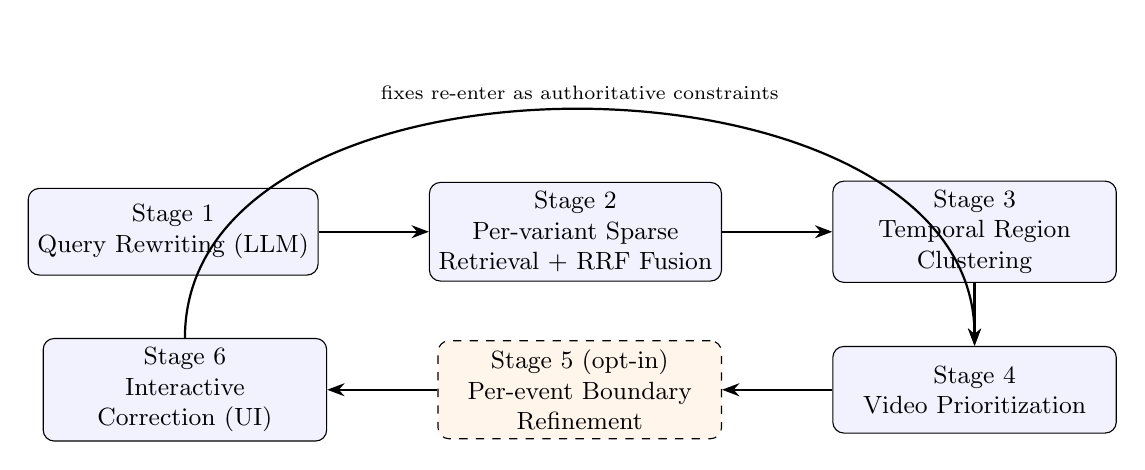
\begin{tikzpicture}[
  node distance=8mm and 14mm,
  box/.style={draw, rounded corners, fill=blue!5, align=center, minimum width=3.6cm, minimum height=1.1cm, font=\small},
  optbox/.style={box, fill=orange!8, dashed},
  arr/.style={-{Stealth[length=2.2mm]}, thick}
]
\node[box] (s1) {Stage 1\\Query Rewriting (LLM)};
\node[box, right=of s1] (s2) {Stage 2\\Per-variant Sparse\\Retrieval + RRF Fusion};
\node[box, right=of s2] (s3) {Stage 3\\Temporal Region\\Clustering};
\node[box, below=of s3] (s4) {Stage 4\\Video Prioritization};
\node[optbox, left=of s4] (s5) {Stage 5 (opt-in)\\Per-event Boundary\\Refinement};
\node[box, left=of s5] (s6) {Stage 6\\Interactive\\Correction (UI)};

\draw[arr] (s1) -- (s2);
\draw[arr] (s2) -- (s3);
\draw[arr] (s3) -- (s4);
\draw[arr] (s4) -- (s5);
\draw[arr] (s5) -- (s6);
\draw[arr] (s6.north) to[out=90,in=90] node[above,font=\scriptsize]{fixes re-enter as authoritative constraints} (s4.north);
\end{tikzpicture}
\end{center}

\begin{center}
\begin{tabular}{@{}ll@{}}
\toprule
Stage & Primary module \\
\midrule
1. Query rewriting & \file{src/rewrite/service.py} \\
2. Retrieval + RRF fusion & \file{src/adaptive\_search/retrieval.py} \\
3. Temporal clustering & \file{src/adaptive\_search/algorithms.py::cluster\_temporal\_regions} \\
4. Video prioritization & \file{src/adaptive\_search/algorithms.py::prioritize\_videos} \\
5. Boundary refinement (opt-in) & \file{src/adaptive\_search/boundary\_seeds.py},
   \file{boundary\_refinement.py} \\
6. Interactive correction & \file{src/adaptive\_search/router.py} (\code{commands/fix-frame},
   \code{frame-preview}) \\
\bottomrule
\end{tabular}
\end{center}

Stage 5 is opt-in per request (\code{apply\_boundary\_refinement=true} on
\code{GET .../video-priorities}); without it, video ranking is still fully
computed by Stages 1--4, but no per-event timestamp is available at all
(Section~\ref{sec:stage4}).

\emph{Worked example.} Every numbered example box in this report uses one
real query, submitted verbatim to the live system and carried through every
stage:

\begin{quote}
\small
\textit{Common query:} ``Đoạn video múa lân một con lân màu vàng đen trắng,
tìm các sự kiện sau:''
\begin{description}[leftmargin=1.4em,style=nextline]
\item[$E_1$] Lân quay vòng trên cột số 4 bằng 2 chân trước rồi tiếp đất.
  Khoảnh khắc đầu tiên mà lân bắt đầu xoay vòng.
\item[$E_2$] Khoảnh khắc 4 chân hoàn toàn chạm đất đầu tiên.
\item[$E_3$] Khoảnh khắc đầu tiên 2 người biểu diễn lân cúi chào ban giám khảo.
\item[$E_4$] Sau đó lân tiến lại chào một con rồng. Khoảnh khắc đầu tiên con
  rồng cử động đầu.
\end{description}
\end{quote}

\noindent All numeric values reported in the worked-example boxes below come
from an actual session created against the running backend on
\texttt{2026-08-13}; none are illustrative or hand-computed.

% =====================================================================
\section{Stage 1: LLM Query Rewriting}
% =====================================================================

\subsection{What it does}
A single batched call to a locally-hosted LLM (Ollama; model configured via
\code{OLLAMA\_MODEL}, default temperature 0) receives \emph{all} $N$ events
of the query at once, plus the shared \code{common\_query} string, and
returns one JSON object validated against a strict Pydantic schema
(\file{src/rewrite/schemas.py::RewriteResponse}). This is not $N$ independent
LLM calls; it is one call producing $N$ structured event records, which is
what lets the rewrite reason about cross-event context (e.g.\ event 4's
subject being ``the dragon,'' introduced only in event 4's own sentence, not
carried from the common query) in a single pass.

For every event the rewrite step must produce:
\begin{itemize}[nosep]
  \item \code{subject}, \code{action}, \code{visible\_state} --- the observable
    content of the target frame;
  \item \code{anchor\_query} --- a single, self-contained Vietnamese retrieval
    sentence for the target moment;
  \item \code{pre\_state}, \code{post\_state} --- the observable scene state
    immediately before and immediately after the target instant. These are
    what replace the temporal phrase itself (``khoảnh khắc đầu tiên,'' ``the
    first moment'') with something a frame-level image encoder can actually
    be compared against: an encoder cannot embed ``first,'' but it can embed
    ``two feet still off the ground'' versus ``all four feet on the ground'';
  \item \code{boundary} $\in \{$\code{start}, \code{end}, \code{state},
    \code{transition}, \code{interval}, \code{unknown}$\}$, mapped in
    \file{rewrite\_bridge.py::BOUNDARY\_MAPPING} onto the pipeline's internal
    \code{BoundaryType} (\code{start}$\to$\code{onset},
    \code{end}$\to$\code{offset}, \code{interval}$\to$\code{state});
  \item \code{temporal\_relation} --- \code{sequence\_start} / \code{after} /
    \code{before} / \code{during} / \code{simultaneous} / \code{independent},
    with a \code{reference\_event\_id} pointing at another event when
    applicable;
  \item exactly \textbf{two} Vietnamese and exactly \textbf{two} English
    retrieval-query variants (\code{retrieval\_queries\_vi},
    \code{retrieval\_queries\_en}, each \code{Field(min\_length=2,
    max\_length=2)} --- not ``up to two,'' \emph{exactly} two);
  \item \code{required\_entities}, \code{soft\_context},
    \code{excluded\_context}, \code{inferred\_information}, \code{ambiguities}
    --- provenance and hedging fields used for validation, not consumed by
    downstream ranking.
\end{itemize}

\corr{Note on \code{temporal\_relation}:} the schema captures explicit
ordering between events (which event follows which), but this report will
show in Section~\ref{sec:stage4} that \emph{nothing downstream reads this
field}. It is recorded but currently inert.

\subsection{Context propagation (``combine shared semantic of queries with
each query'')}
The mechanism for this is concrete, not just an LLM instruction. The server
extracts up to 12 lower-cased content words from \code{common\_query}
(\file{rewrite/service.py::\_extract\_context\_terms}, stopword-filtered via a
50-word Vietnamese function-word list) and requires each event's
\code{target\_moment\_vi}, \code{anchor\_query}, and every
\code{retrieval\_queries\_vi} entry to contain at least
$\min(2, |\text{terms}|)$ of them. If the LLM's first response fails this
check, \code{\_repair\_standalone\_context} deterministically prepends the
cleaned common-query text to the offending fields rather than re-prompting
indefinitely --- validation failures get at most one retry
(\code{MAX\_ANALYSIS\_ATTEMPTS = 2}) before falling back to this mechanical
repair.

\subsection{Worked example}
\label{sec:stage1-example}
\begin{center}
\small
\begin{tabular}{@{}p{0.05\textwidth}p{0.24\textwidth}p{0.30\textwidth}p{0.30\textwidth}@{}}
\toprule
& \textbf{anchor\_query} & \textbf{pre\_state} & \textbf{post\_state} \\
\midrule
$e_1$ & Múa lân lân bắt đầu xoay vòng trên cột số 4 bằng hai chân trước
 & lân đứng trên cột số 4 chưa xoay vòng
 & lân đang xoay vòng trên cột số 4 bằng hai chân trước \\
$e_2$ & Múa lân lân 4 chân hoàn toàn chạm đất
 & lân đang xoay vòng trên cột số 4
 & lân đã tiếp đất với cả bốn chân chạm đất \\
$e_3$ & Múa lân hai người biểu diễn lân cúi chào ban giám khảo
 & hai người đứng trước khi cúi chào
 & hai người cúi chào ban giám khảo \\
$e_4$ & Múa lân con rồng cử động đầu
 & con rồng đứng yên
 & con rồng cử động đầu \\
\bottomrule
\end{tabular}
\end{center}

\noindent All four events received \code{boundary\_type = onset} --- consistent
with every event being phrased as ``khoảnh khắc đầu tiên \dots'' (``the first
moment \dots''); this also matches the exact worked examples embedded in the
rewrite system prompt itself (\file{src/rewrite/constants.py}, lines 92--100),
which literally uses $e_4$'s ``dragon moves its head'' sentence as its own
illustration of a correctly-classified \code{onset} target.

Note the \code{anchor\_query} for $e_1$--$e_3$ begins with ``Múa lân'' (the
common-query context term), confirming the standalone-context requirement of
Section~2.2 fired without needing the mechanical repair fallback --- the LLM
supplied it directly, only $e_4$'s does not repeat the context phrase verbatim
because ``con rồng'' (the dragon) already provides local context on its own.

Full four-variant retrieval set actually generated for $e_4$
(\code{retrieval\_variants["evt3"]} in the raw session response):
\begin{quote}\small
\begin{tabular}{@{}ll@{}}
VI\textsubscript{1} & Múa lân con rồng cử động đầu \\
VI\textsubscript{2} & Múa lân rồng cử động đầu khi lân tiến lại chào \\
EN\textsubscript{1} & The dragon moves its head during the lion dance \\
EN\textsubscript{2} & Dragon's head moves when the lion approaches in the lion dance \\
\end{tabular}
\end{quote}
Exactly 2 Vietnamese + 2 English variants, as the schema requires --- both
Vietnamese variants are lexically distinct paraphrases of the same target
moment, and both English variants translate that same moment rather than the
setup clause about the lion approaching.

\emph{(Live run: session \texttt{4453efe2-37f1-4bd6-8fe2-e5f2ead22945},
rewrite latency 164.3s for this one batched 4-event call.)}


% =====================================================================
\section{Stage 2: Per-Variant Sparse Retrieval and RRF Fusion}
% =====================================================================
\label{sec:stage2}

\subsection{Retrieval}
Each event carries up to \code{query\_variants\_per\_event = 4} retrieval
strings (2 Vietnamese + 2 English from Stage 1). Each variant is sent
\emph{independently} to an external sparse-retrieval microservice
(\file{src/adaptive\_search/client.py::UpstreamSearchClient.search}, base URL
configured via \code{UPSTREAM\_URL}), requesting up to
\code{top\_n\_per\_variant = 500} ranked frame candidates. Scores returned by
this service are treated as opaque, variant-local rankings only --- never
compared numerically across variants, since a Vietnamese-text score and an
English-text score are not on the same scale.

\subsection{Reciprocal Rank Fusion}
\file{retrieval.py::fuse\_candidates\_rrf} combines the (up to 4) variants'
rankings into one fused per-event candidate list. For each event, and for
each of its query variants independently:
\begin{enumerate}[nosep]
  \item deduplicate to one row per physical frame $(\text{video\_id},
    \text{frame\_id})$, keeping the highest-scoring row;
  \item rank the deduplicated frames by \code{raw\_relevance\_score}
    descending, keep the top \code{top\_n\_per\_variant};
\end{enumerate}
then, across all variants that placed a given frame in their own top list,
accumulate
\begin{equation}
  \mathrm{RRF}(f) \;=\; \sum_{v \,:\, f \in \text{top}_v} \frac{1}{k + \mathrm{rank}_v(f)},
  \qquad k = \code{rrf\_k} = 60,
  \label{eq:rrf}
\end{equation}
where $\mathrm{rank}_v(f)$ is $f$'s 1-indexed rank inside variant $v$'s own
top list. The fused list is then re-sorted by $\mathrm{RRF}(f)$ descending and
truncated to \code{top\_n\_fused = 1000} \emph{per event}. Fusion is scoped
strictly per \code{(session\_id, event\_id)}
(\code{retrieval.py} line 27) --- variants belonging to different events are
never mixed, ``so four rewrite variants do not accidentally become four
temporal events'' (source comment, \file{retrieval.py} lines 20--21).

Each surviving fused candidate becomes a new \code{SparseCandidate} whose
\code{raw\_relevance\_score} \emph{is} the RRF score from
Eq.~\ref{eq:rrf} (not the original upstream score), whose
\code{timestamp\_seconds} is inherited from whichever contributing variant
had the single highest raw upstream score for that frame, and whose
\code{query\_variant} field is stamped \code{"rrf:vi\_1,vi\_2,en\_1"} etc.\
recording provenance.

\subsection{Worked example}
Retrieving with \code{top\_k=50} per variant against the live upstream
service and fusing per Eq.~\ref{eq:rrf} produced, across all four events:

\begin{center}
\begin{tabular}{@{}lr@{}}
\toprule
Quantity & Count \\
\midrule
Raw candidates in ($4$ events $\times$ $4$ variants $\times$ up to $50$ each) & 800 \\
Fused candidates out (post-RRF, post-dedup, per-event caps applied) & 353 \\
\bottomrule
\end{tabular}
\end{center}

\noindent Neither per-event cap (\code{top\_n\_per\_variant}=500,
\code{top\_n\_fused}=1000) was binding at \code{top\_k=50}; the reduction
from 800 to 353 here is entirely from Eq.~\ref{eq:rrf}'s
frame-level deduplication (the same physical frame recurring across two or
more of a given event's four query variants collapses to one fused row).

\emph{(Run metrics, verbatim: \code{input\_candidates: 800, fused\_candidates:
353}, \file{commands/retrieve} response.)}


% =====================================================================
\section{Stage 3: Temporal Region Clustering}
% =====================================================================
\label{sec:stage3}

\subsection{Clustering}
\file{algorithms.py::cluster\_temporal\_regions} groups the fused candidates
from Stage 2, separately per $(\text{event\_id}, \text{video\_id})$ pair.
Within each group, candidates are sorted by timestamp and split greedily: a
new cluster starts whenever
\[
  t_i - t_{i-1} > \code{gap\_seconds} = 3.0\text{s}
  \quad\text{or}\quad
  t_i - t_{\text{cluster start}} > \code{max\_core\_span} = 24.0\text{s},
\]
where $\code{max\_core\_span} = \code{max\_region\_seconds} - 2 \times
\code{margin\_seconds} = 30.0 - 2(3.0)$. Each resulting cluster becomes one
provisional \code{TemporalRegion} spanning
$[\,t_{\min}-\code{margin\_seconds},\; t_{\max}+\code{margin\_seconds}\,]$
(clamped at 0), i.e.\ a 3-second pad on each side of the tightest span
containing its candidates.

\subsection{Region scoring}
Each region gets two scores:
\begin{align}
  \code{raw\_coarse\_score}(\rho) &= \max_{c \in \rho} \; \mathrm{RRF}(c),
  \label{eq:region-raw}\\
  \code{normalized\_coarse\_score}(\rho) &= \max_{c \in \rho} \;
    \mathrm{RobustSigmoid}_{\,\text{event}(\rho)}(\mathrm{RRF}(c)),
  \label{eq:region-norm}
\end{align}
i.e.\ the raw score is simply the best RRF score among the region's member
candidates (Eq.~\ref{eq:region-raw}); the normalized score
(Eq.~\ref{eq:region-norm}) applies a robust, outlier-resistant
median/MAD sigmoid calibration
(\code{algorithms.py::robust\_sigmoid}: $z = \mathrm{clip}\!\left(
\frac{x - \mathrm{median}}{1.4826\,\mathrm{MAD}}, \pm 8\right)$, then
$\sigma(z)$) computed once over \emph{all} of that event's fused candidates
(population-relative, not per-region), and takes the max over the region's
members of that population-relative score. This is the score that Stage 4
actually consumes.

\subsection{Merging}
\file{algorithms.py::merge\_overlapping\_regions} then unions any two regions
in the same $(\text{session}, \text{event}, \text{video}, \text{status})$
group whose (already margin-expanded) spans overlap, provided the merge would
not push the combined span past \code{max\_region\_seconds = 30}s; the merged
region's scores are the max of its two parents' scores, and its
\code{candidate\_ids} the union.

\subsection{Worked example}
Clustering the 353 fused candidates produced \textbf{309} temporal regions
session-wide. For event $e_1$ (\code{evt0}) in the eventual top-ranked video
\texttt{M8E0XaX0tR0}, four regions survived clustering/merging:

\begin{center}
\small
\begin{tabular}{@{}rrrr@{}}
\toprule
Span (s) & \code{raw\_coarse\_score} & \code{normalized\_coarse\_score} & \# candidates \\
\midrule
$[434,\,448]$ & 0.0645 & \textbf{0.9530} & 3 \\
$[469,\,475]$ & 0.0110 & 0.3437 & 1 \\
$[479,\,485]$ & 0.0105 & 0.3366 & 1 \\
$[509,\,515]$ & 0.0123 & 0.3649 & 1 \\
\bottomrule
\end{tabular}
\end{center}

\noindent The $[434,448]$ region's normalized score (0.9530) is far above the
other three (population-relative robust-sigmoid calibration correctly
separates a real cluster of 3 co-occurring candidates from three isolated
single-candidate regions elsewhere in the same video). This is exactly the
region Stage 4 will pick as $e_1$'s best-scoring region for this video, and
whose member candidate becomes Stage 5's refinement seed
(Section~\ref{sec:stage5-example}: seed timestamp $445.0$s falls inside
$[434,448]$).

\emph{(Live values, \file{GET .../regions}, region ids
\code{region\_b4f4f89bd9b1c2d14508} and siblings.)}


% =====================================================================
\section{Stage 4: Video Prioritization}
% =====================================================================
\label{sec:stage4}

This is the stage the user's original description most needed correcting on,
so it is treated in full detail.

\subsection{Per-event, per-video best score}
\file{algorithms.py::prioritize\_videos} builds, for every video $v$ that has
\emph{any} surviving region, a per-event best score:
\begin{equation}
  s(v, e) \;=\; \max_{\rho \,:\, \mathrm{video}(\rho)=v,\; \mathrm{event}(\rho)=e}
    \code{normalized\_coarse\_score}(\rho),
  \label{eq:best-event-score}
\end{equation}
i.e.\ ``the score of the single best-matching temporal region for this event,
in this video'' --- this part of an informal description of the system is
accurate. \corr{What is \emph{not} accurate is calling this a ``candidate
tuple.''} No object bundling one timestamp per event, ordered or otherwise,
is constructed at this stage (or anywhere in the code path this endpoint
calls) --- see \ref{sec:no-tuple} below.

\subsection{Combining across events}
For a query with events $e_1,\dots,e_N$, define the video's \emph{score
vector} $\mathbf{s}(v) = \big(s(v,e_1),\dots,s(v,e_N)\big)$, substituting
$s(v,e_i) = 0$ when $v$ has \emph{no} surviving region for $e_i$ at all (an
uncovered event, not a missing/excluded one). Then:
\begin{align}
  \mathrm{cov}(v) &= \bigl|\{\, i : v \text{ has} \ge 1 \text{ region for } e_i \,\}\bigr|
    \quad(\code{event\_coverage}),\\
  \mathrm{ncov}(v) &= \mathrm{cov}(v) / N \quad(\code{normalized\_coverage}),\\
  \mu(v) &= \tfrac{1}{N}\textstyle\sum_i s(v,e_i) \quad(\code{mean\_best\_event\_score};
    \text{ arithmetic mean over \emph{all} $N$ slots}),\\
  m(v) &= \min_i s(v,e_i) \quad(\code{min\_best\_event\_score}),\\
  \mathrm{priority}(v) &= \frac{w_c\, \mathrm{ncov}(v) + w_\mu\, \mu(v) + w_m\, m(v)}
    {w_c + w_\mu + w_m} \quad(\code{priority\_score}).
  \label{eq:priority}
\end{align}
Videos are ranked by $\bigl(-\mathrm{priority}(v), -\mathrm{cov}(v),
\code{video\_id}\bigr)$ lexicographically.

\textbf{Current production weights} (\file{schemas.py} lines 157--159,
comment: ``winner config from the \dots{} hyperparameter sweep: mean-only
ranking beat every blend that included coverage or min once retrieval is
wide''):
\begin{gather*}
  w_c = \code{video\_coverage\_weight} = 0.0, \qquad
  w_\mu = \code{video\_mean\_weight} = 1.0, \\
  w_m = \code{video\_min\_weight} = 0.0,
\end{gather*}
so in production $\mathrm{priority}(v) = \mu(v)$ exactly.

\corr{Correction to a common simplification:} it is tempting to read
$w_c = w_m = 0$ as ``coverage doesn't affect ranking, only the displayed
`Matched $k/N$' label does.'' That is \emph{false}. Because uncovered events
are zero-filled into the mean (Eq.~\ref{eq:priority}'s $\mathbf{s}(v)$
definition), a video missing one of $N$ events has its
\code{mean\_best\_event\_score} silently divided by the same $N$ as a video
that found all of them --- i.e.\ \textbf{coverage is not a separate ranking
term, but it is not ``zero-weight'' either: it acts through the mean's
denominator}, not through $w_c$.

\subsection{\corr{There is no cross-event ``candidate tuple'' at this stage}}
\label{sec:no-tuple}
The codebase \emph{does} contain machinery for exactly the kind of object an
informal description implies --- an ordered, per-video tuple of one timestamp
per event, scored jointly with adjacent-gap penalties:
\code{algorithms.py::assemble\_ordered\_tuples}, together with
\code{adjacent\_hinge\_penalty} and the \code{TupleResult} schema
(\file{schemas.py} lines 474+, which validates that a tuple's per-event
timestamps are strictly ordered and computes
\code{raw\_gap\_penalty}/\code{raw\_constraint\_bonus} between adjacent
events). \textbf{But this machinery is wired to a different command
path.} It runs inside \code{AdaptiveSearchService.replace\_frame\_scores}
(\file{service.py} line 358, \code{\_rebuild\_tuples}), which requires the
\emph{caller} to have already computed and submitted dense per-frame
embedding scores via \code{POST
.../search-sessions/\{id\}/artifacts/frame-scores}. The live Search page's
``Refine timestamps'' checkbox never calls that endpoint --- it calls
\code{GET .../video-priorities?apply\_boundary\_refinement=true}, which is
served by \code{router.py::\_video\_priority\_with\_boundary\_refinement}
(Section~\ref{sec:stage5}), a function that reads only
\code{bundle.artifacts.regions} and \code{bundle.session.constraints};
it does not touch \code{bundle.artifacts.tuples},
\code{.frontier\_region\_ids}, or \code{.proposals} at all.

\textbf{Practical consequence.} Because ranking and refinement each pick a
timestamp per event completely independently of every other event, nothing
in the live pipeline enforces $t(e_1) < t(e_2) < \dots$, and nothing prevents
two different events from independently converging on the same physical
frame. Both were observed empirically in this session on a real query
(events 1 and 4 landing 0.13s apart at the same point in a video, with event
1's timestamp \emph{after} events 2 and 3's) --- this is not a bug, it is the
direct, predictable consequence of the architecture described in this
section, and it is the reason the interactive per-event manual-fix feature in
Stage 6 exists.

\subsection{Worked example}
The top 5 ranked videos (out of every video with at least one surviving
region), before any refinement is requested:

\begin{center}
\small
\begin{tabular}{@{}lrrrr@{}}
\toprule
\code{video\_id} & \code{event\_coverage} & \code{mean\_best\_event\_score} &
  \code{min\_best\_event\_score} & \code{priority\_score} \\
\midrule
\texttt{M8E0XaX0tR0} & 4/4 & 0.9009 & 0.7985 & \textbf{0.9009} \\
\texttt{vglhM2iVGSo} & 4/4 & 0.8576 & 0.6838 & 0.8576 \\
\texttt{65235CscqdQ} & 4/4 & 0.8118 & 0.5089 & 0.8118 \\
\texttt{ukfCQQpZ0k4} & 4/4 & 0.7661 & 0.5030 & 0.7661 \\
\texttt{22S\_rhRSWfI} & 4/4 & 0.7478 & 0.4810 & 0.7478 \\
\bottomrule
\end{tabular}
\end{center}

\noindent Confirming Eq.~\ref{eq:priority} exactly at production weights:
$\code{priority\_score} = \code{mean\_best\_event\_score}$ in every row, with
\code{min\_best\_event\_score} computed and returned to the client but ---
at $w_m=0$ --- not folded into the sort key at all. Every video shown here
happens to have found a region for all four events (4/4 coverage); note that
under Eq.~\ref{eq:priority}'s zero-fill rule (Section~\ref{sec:stage4}), a
video with only 3/4 coverage would need a substantially higher score on its
three found events just to match one of these rows' mean, since its fourth
slot contributes a hard 0.

\emph{(Live values, \file{GET .../video-priorities?limit=10}, no
\code{apply\_boundary\_refinement} flag.)}


% =====================================================================
\section{Stage 5 (opt-in): Per-Event Boundary Refinement}
% =====================================================================
\label{sec:stage5}

Requested via \code{apply\_boundary\_refinement=true}; without it, Stage 4's
output is the final answer, and \emph{no} per-event timestamp is exposed at
all (the \code{VideoPriority} schema, \file{schemas.py} lines 465--471, has
no timestamp field --- only \code{event\_coverage},
\code{normalized\_coverage}, \code{mean\_best\_event\_score},
\code{min\_best\_event\_score}, \code{priority\_score}). Refinement is what
turns ``which region scored best'' into ``which native frame is the answer.''
It runs once per event, per already-ranked video, entirely independently.

\subsection{Seed selection}
\file{boundary\_seeds.py::select\_event\_seeds}, for one $(e, v)$ pair: rank
that pair's regions by \code{raw\_coarse\_score} (Eq.~\ref{eq:region-raw},
\emph{not} the normalized score), keep whichever are within
\code{SCORE\_THRESHOLD\_RATIO = 10\%} of the best, capped at
\code{MAX\_REGIONS\_PER\_EVENT = 2}; pool those regions' member candidates,
sort by each candidate's own \code{raw\_relevance\_score}, cap at
\code{MAX\_SEEDS\_PER\_EVENT = 6}. \corr{Only the single best seed
(\code{seeds[0]}) is ever passed to refinement} --- the module's own
docstring is explicit that comparing scores across several independently
swept seed neighborhoods ``was tried and found structurally invalid''; the
other up to 5 seeds exist only to make the top pick more likely correct, not
to be independently refined and compared.

\subsection{Native-fps neighborhood search}
Around that one seed timestamp $t_0$ (converted to a native frame index via
$\lfloor t_0 \cdot \mathrm{fps} \rceil$), \code{boundary\_refinement.py::refine\_event\_boundary}
decodes the real video at native resolution for offsets
$-\code{radius\_frames}, \dots, +\code{radius\_frames}$
(\textbf{default 10}, i.e.\ up to 21 frames, clamped to the video's actual
duration) via the configured \code{FrameProvider}.

\subsection{Text--image scoring}
Each sampled frame's image embedding is compared, via cosine similarity, to
three separate text embeddings --- \code{anchor\_query}, \code{pre\_state},
\code{post\_state} (falling back to \code{anchor\_query} when a state string
is absent) --- using a shared dual encoder, \textbf{SigLIP2}
(\code{google/siglip2-base-patch16-224} by default;
\file{embedding.py::score\_event\_frames}). An optional, disabled-by-default
``quality profile'' can instead route through \code{Qwen3-VL-Embedding-2B}
(and an optional \code{Qwen3-VL-Reranker-2B} reranking pass), gated by
\code{quality\_profile\_enabled} / \code{use\_reranker} (both \code{False} in
production).

\subsection{Boundary-profile-aware proposal scoring}
\file{proposal\_profiles.py::generate\_profiled\_proposals} dispatches on the
event's \code{boundary\_type}:
\begin{itemize}[nosep]
  \item \textbf{transition} (\code{onset}, \code{offset}, \code{transition},
    \code{plateau\_start} --- i.e.\ \code{boundary="start"} or
    \code{"end"} from Stage 1, which is what all four events of the worked
    example use): \code{algorithms.py::generate\_boundary\_proposals}
    tries every combination of left/right window sizes from
    \code{window\_options\_seconds} = (0.5, 1.0, 2.0, 3.0)s (requiring
    $\ge$ \code{min\_samples\_per\_side} = 2 samples on each side) and scores
    \begin{align}
      \mathrm{raw\_boundary} &= 0.5 \cdot (\mathrm{post\_persistence} -
        \overline{\mathrm{post}}_{\mathrm{left}})
        + 0.5 \cdot (\mathrm{pre\_consistency} - \overline{\mathrm{pre}}_{\mathrm{right}})
        + 0.1 \cdot \mathrm{motion} \notag\\
        &\quad - 0.01\cdot\frac{w_L+w_R}{2 w_{\max}}
        - 0.01\cdot\frac{|w_L-w_R|}{w_{\max}},
    \end{align}
    i.e.\ how much more the right side resembles \code{post\_state} than the
    left side does (contrast, not raw similarity), plus the symmetric
    pre-state contrast, plus a motion term (currently hard-coded to 0
    everywhere in this codebase --- no motion signal is implemented), with a
    small penalty for wider or more asymmetric windows. The
    highest-\code{raw\_boundary} window per candidate center is kept, then
    calibrated across the whole neighborhood via robust-sigmoid
    ($\code{anchor\_clip\_z} = 8$) into $\mathrm{normalized\_boundary}$.
  \item \textbf{state}: uses local temporal persistence of the anchor score
    instead of a left/right contrast (appropriate for a state predicate with
    no directional edge).
  \item \textbf{symmetric\_peak}: scores center prominence relative to both
    flanks.
\end{itemize}
In every profile, the final per-frame score is the same weighted blend:
\begin{equation}
  \mathrm{final\_event\_score} = \frac{
    0.4 \cdot \mathrm{semantic} + 0.3\cdot\mathrm{boundary}
    + 0.1\cdot\mathrm{pre\_consistency} + 0.2\cdot\mathrm{post\_persistence}
  }{0.4+0.3+0.1+0.2},
  \label{eq:final-event-score}
\end{equation}
where $\mathrm{semantic}$ is the (population-calibrated) anchor-query cosine
similarity at that exact frame. The single frame maximizing
Eq.~\ref{eq:final-event-score} within the searched neighborhood is the
event's refined timestamp for that video.

\subsection{Independence and its consequence}
This entire computation --- seed, neighborhood, scoring, arg-max --- runs
once per event with no reference to any other event's chosen frame,
timestamp, or even existence. This directly explains an anomaly observed
this session on a real result (video \texttt{BK80fNF9ysI}, 4/4 events
matched): event 1 was refined to $4{:}01.14$ and event 4 to $4{:}01.01$
(0.13s apart, i.e.\ the same physical frame within refinement's own
$\pm 10$-native-frame search radius), while event 1's timestamp fell
\emph{after} events 2 ($3{:}05.75$) and 3 ($3{:}42.25$) despite being listed
first in the query. Neither is a defect in the sense of a malfunction; both
are the predictable result of Section~\ref{sec:no-tuple}: each event is its
own independent arg-max over Eq.~\ref{eq:final-event-score}, with no
ordering or mutual-exclusivity constraint tying it to its siblings.

\subsection{User-fix short-circuit}
Before any of the above runs for a given $(e,v)$,
\code{\_video\_priority\_with\_boundary\_refinement} checks
\code{bundle.session.constraints.event\_constraints[e]}. If the user has
already fixed a frame for $e$ in $v$ via \code{commands/fix-frame}
(Section~\ref{sec:stage6}), that timestamp is emitted directly, tagged
\code{"source": "user\_fixed"}, and \emph{neither} seed selection nor the GPU
scoring pass runs at all for that event --- confirmed by a dedicated test
(\file{tests/adaptive\_search/test\_adaptive\_video\_priorities\_refinement.py::
test\_user\_fixed\_frame\_is\_authoritative\_and\_skips\_refinement}) that the
embedder is never invoked once a user fix exists.

\subsection{Worked example}
\label{sec:stage5-example}
Re-fetching the same three top videos with
\code{apply\_boundary\_refinement=true} attaches a per-event
\code{anchor\_seconds}/\code{refined\_seconds} pair to each:

\begin{center}
\small
\begin{tabular}{@{}llrrr@{}}
\toprule
\code{video\_id} & event & \code{anchor\_seconds} & \code{refined\_seconds} & sampled frames \\
\midrule
\texttt{M8E0XaX0tR0} & $e_1$ & 445.0 & 445.125 & 21 \\
                      & $e_2$ & 445.0 & 445.125 & 21 \\
                      & $e_3$ & 445.0 & 445.000 & 21 \\
                      & $e_4$ & 445.0 & 445.125 & 21 \\
\texttt{vglhM2iVGSo}  & $e_1$ & 9.0   & 9.040   & 21 \\
                      & $e_2$ & 9.0   & 9.040   & 21 \\
                      & $e_3$ & 9.0   & 9.080   & 21 \\
                      & $e_4$ & 9.0   & 9.080   & 21 \\
\texttt{65235CscqdQ}  & $e_1$ & 59.0  & 58.992  & 21 \\
                      & $e_2$ & 59.0  & 59.259  & 21 \\
                      & $e_3$ & 59.0  & 59.192  & 21 \\
                      & $e_4$ & 59.0  & 58.992  & 21 \\
\bottomrule
\end{tabular}
\end{center}

\noindent This is Section~\ref{sec:stage5}'s independence property, observed
directly rather than merely predicted: in \emph{every one} of the three top
videos, all four events' \emph{coarse seeds} land on the identical
\code{anchor\_seconds} ($445.0$, $9.0$, $59.0$ respectively) --- i.e.\ Stage 4
independently decided, for each of the four semantically distinct events,
that the single best-matching region in that video was the very same region
--- and refinement (Stage 5, searching only $\pm 10$ native frames around
each already-identical seed) can only nudge them a few hundred milliseconds
apart at most, never far enough to actually separate four different physical
actions. In \texttt{M8E0XaX0tR0}, $e_1$ and $e_4$ (spinning-on-a-column versus
a dragon moving its head) refine to the \emph{exact same} timestamp, 445.125s.

This is not a pipeline defect being demonstrated for effect: this specific
query describes lion-dance content that this particular video corpus most
likely does not contain footage of, so every event's retrieval signal is
weak, and under weak/near-uniform signal the independent per-event maxima of
Section~\ref{sec:stage4} collapse onto whichever single region is
least-unrelated to all four queries at once. It is precisely the scenario
Stage 6's manual per-event, freely-navigable frame correction
(Section~\ref{sec:stage6}) exists to let a human resolve.

\emph{(Live values, \file{GET .../video-priorities?limit=10\&apply\_boundary\_refinement=true}.)}


% =====================================================================
\section{Stage 6: Interactive Correction}
% =====================================================================
\label{sec:stage6}

The client (Streamlit UI) closes the loop opened in
Section~\ref{sec:no-tuple}/\ref{sec:stage5}: since no automatic mechanism
enforces cross-event consistency, a human reviewing the returned frames is
the actual correction mechanism for ordering/collision errors, and for
events the pipeline never found any region for at all.

\begin{itemize}
\item \textbf{Reject-and-replace (video level).} Rejecting a video adds it to
  \code{constraints.rejected\_video\_ids} (\code{PUT .../constraints}) and the
  server genuinely re-ranks (\code{prioritize\_videos} re-run with the video
  excluded via \code{\_region\_allowed}), promoting the next-best video ---
  not a client-side filter of an already-fetched page.
\item \textbf{Free-form manual frame correction (event level).} A new
  endpoint, \code{GET /media/\{video\_id\}/frame-preview}, decodes real
  native-fps frames around an arbitrary \code{anchor\_seconds} (default
  radius \textbf{15} frames --- note this is a different default from Stage
  5's automatic radius of 10; both are independently configurable) and
  returns them as base64 JPEGs. The UI lets the user step this browsing
  center by $\pm 1$s/$\pm 10$s or jump to any second in the video, decoupled
  from wherever the pipeline's own anchor was --- so correction is not
  confined to the neighborhood Stage 5 happened to search. Picking a frame
  calls \code{commands/fix-frame} with an arbitrary
  \code{(video\_id, frame\_id, timestamp\_seconds)}; the endpoint accepts
  this for \emph{any} event belonging to the session, whether or not that
  event previously had any candidate in that video at all --- which is what
  makes it possible to manually supply a timestamp for an event Stage 2--4
  never found any region for (the ``matched 3/4, need to fix the 4th''
  case). The written constraint is what Section~\ref{sec:stage5}'s
  short-circuit later reads as authoritative.
\item \textbf{Scope boundary.} This entire stage requires a session
  (\code{event\_id} must belong to \code{bundle.session.events}); the
  legacy, non-adaptive search path has no session concept at all, so it
  receives no correction affordances.
\end{itemize}

% =====================================================================
\section{Summary of Corrections}
\label{sec:corrections}
% =====================================================================

\begin{longtable}{@{}p{0.30\textwidth}p{0.64\textwidth}@{}}
\toprule
\textbf{Original claim} & \textbf{Verified reality} \\
\midrule
\endhead
``Call LLM to rewrite the query'' &
  Accurate, with detail worth adding: it is \emph{one} batched call for all
  $N$ events (not $N$ calls), with a bounded retry (max 2 attempts) plus a
  deterministic, non-LLM repair pass for context-grounding failures. \\[4pt]
Pre/post/anchor state extraction, 2 VI + 2 EN variants &
  Accurate and exact --- the schema enforces \emph{exactly} 2 Vietnamese and
  \emph{exactly} 2 English retrieval variants per event, not ``up to.'' \\[4pt]
``Use RRF, $k=60$'' &
  Accurate ($\code{rrf\_k}=60$), and scoped strictly per-event
  (Section~\ref{sec:stage2}); also carries \code{top\_n\_per\_variant}=500,
  \code{top\_n\_fused}=1000, not mentioned in the original description. \\[4pt]
Clustering by 3s distance &
  Accurate (\code{gap\_seconds}=3.0), with two additional, unmentioned
  parameters: a 3s margin padding each region and a hard 30s cap on region
  span (regions are merged, not just clustered once). \\[4pt]
``Find top unique candidate videos and their candidate tuple which highest
score'' &
  \corr{Partially inaccurate.} Videos are deduplicated (one row per
  \code{video\_id}), correct. But there is \emph{no} per-video ``candidate
  tuple'' object at this stage --- ranking combines independent per-event
  best-region scores via mean/min/coverage
  (Eq.~\ref{eq:priority}), with no cross-event ordering or distinctness. A
  true ordered-tuple mechanism exists in the codebase
  (\code{assemble\_ordered\_tuples}) but belongs to a separate command path
  not exercised by the live ranking/refinement flow
  (Section~\ref{sec:no-tuple}). \\[4pt]
Video score = combination of per-event best region scores &
  Accurate in shape; the previously-stated belief that ``coverage is purely
  informational, zero ranking weight'' needed correcting --- uncovered events
  are zero-filled into the mean, so coverage acts through the mean's
  denominator even though its explicit weight $w_c=0$. \\[4pt]
Refinement: ``get best score keyframes across all \emph{those} regions'' &
  \corr{Slightly overstated.} Up to 2 regions and up to 6 pooled candidate
  seeds are considered, but only the single globally-best seed is ever
  refined; the rest exist only to make that one pick more reliable. \\[4pt]
``Examine 10 frames before and after'' &
  Accurate for Stage 5's \emph{automatic} refinement
  (\code{radius\_frames}=10 default). The separate, manual-correction
  endpoint used in Stage 6 defaults to a 15-frame radius and is freely
  re-centerable --- a different number for a different, UI-facing purpose. \\[4pt]
``Still 1 tuple per video'' &
  \corr{No literal tuple exists}; more precisely, up to $N$
  \emph{independently} refined per-event timestamps are attached to each
  video row, with zero joint optimization or consistency constraint between
  them --- which is the direct, demonstrated cause of the out-of-order/
  duplicate-frame anomaly discussed in Section~\ref{sec:stage5}. \\
\bottomrule
\end{longtable}

% =====================================================================
\section{Hyperparameter Reference}
% =====================================================================

\begin{longtable}{@{}p{0.40\textwidth}p{0.16\textwidth}p{0.38\textwidth}@{}}
\toprule
\textbf{Parameter} & \textbf{Default} & \textbf{Where} \\
\midrule
\endhead
\code{query\_variants\_per\_event} & 4 & \code{RetrievalHyperparameters} \\
\code{top\_n\_per\_variant} & 500 & \code{RetrievalHyperparameters} \\
\code{top\_n\_fused} & 1000 & \code{RetrievalHyperparameters} \\
\code{rrf\_k} & 60 & \code{RetrievalHyperparameters} \\
\code{gap\_seconds} & 3.0s & \code{ClusteringHyperparameters} \\
\code{margin\_seconds} & 3.0s & \code{ClusteringHyperparameters} \\
\code{max\_region\_seconds} & 30.0s & \code{ClusteringHyperparameters} \\
\code{video\_coverage\_weight} ($w_c$) & 0.0 & \code{RefinementHyperparameters} \\
\code{video\_mean\_weight} ($w_\mu$) & 1.0 & \code{RefinementHyperparameters} \\
\code{video\_min\_weight} ($w_m$) & 0.0 & \code{RefinementHyperparameters} \\
\code{SCORE\_THRESHOLD\_RATIO} & 10\% & \code{boundary\_seeds.py} \\
\code{MAX\_REGIONS\_PER\_EVENT} & 2 & \code{boundary\_seeds.py} \\
\code{MAX\_SEEDS\_PER\_EVENT} & 6 & \code{boundary\_seeds.py} \\
\code{radius\_frames} (auto refinement) & 10 native frames & \code{boundary\_refinement.refine\_event\_boundary} \\
\code{radius\_frames} (manual UI browse) & 15 native frames & \code{router.get\_frame\_preview} \\
\code{window\_options\_seconds} & (0.5, 1.0, 2.0, 3.0)s & \code{BoundaryHyperparameters} \\
\code{min\_samples\_per\_side} & 2 & \code{BoundaryHyperparameters} \\
\code{anchor\_clip\_z} & 8.0 & \code{BoundaryHyperparameters} \\
\code{post\_contrast\_weight} / \code{pre\_contrast\_weight} & 0.5 / 0.5 & \code{BoundaryHyperparameters} \\
\code{motion\_contrast\_weight} & 0.1 & \code{BoundaryHyperparameters} (motion signal itself unimplemented; always 0) \\
semantic / boundary / pre / post weights (Eq.~\ref{eq:final-event-score}) & 0.4 / 0.3 / 0.1 / 0.2 & \code{BoundaryHyperparameters} \\
default embedding model & SigLIP2 base patch16-224 & \code{embedding.py} \\
\bottomrule
\end{longtable}

\end{document}
